\section{\name's Utility Regime}

\label{s:deploy}
%\radhika{need a better title?}

\begin{figure*}
    \centering
    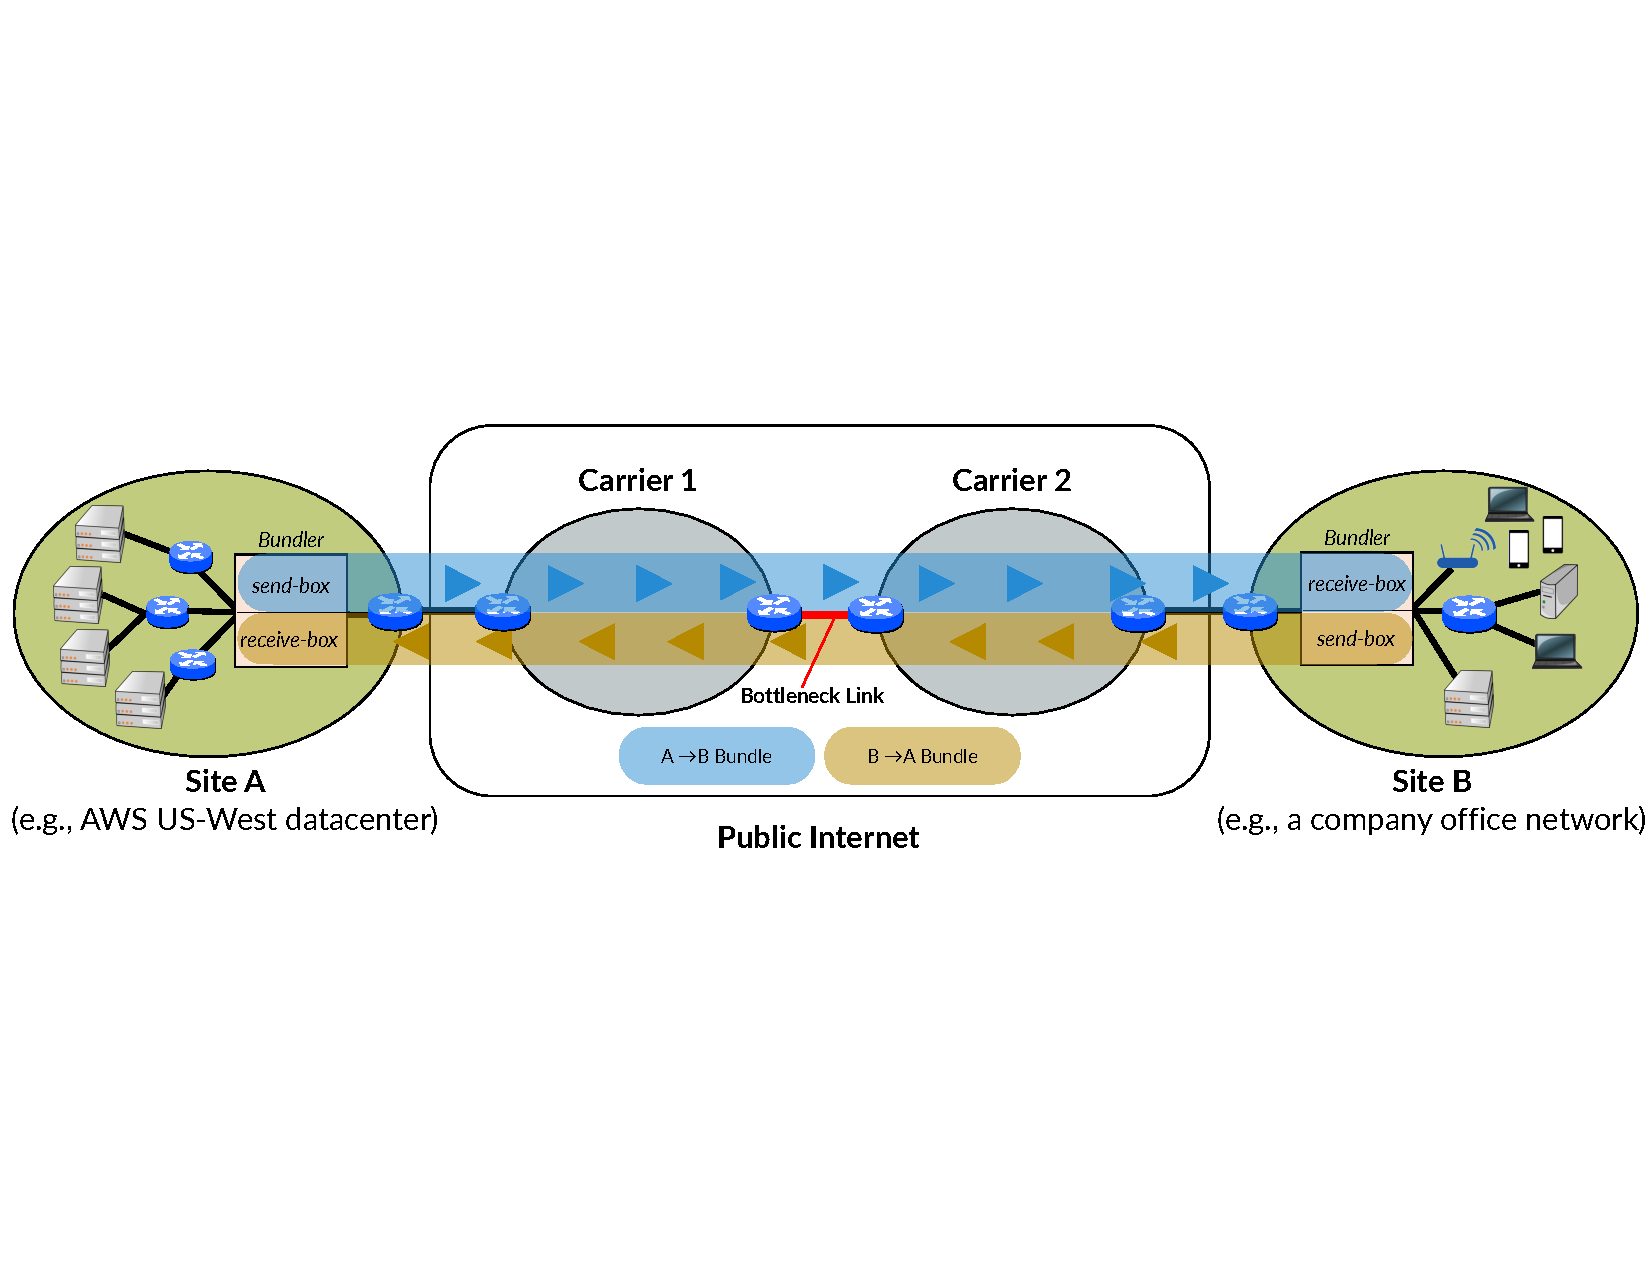
\includegraphics[width=\textwidth]{img/deployment-arch.pdf}
    \caption{An example deployment scenario for \name. 
    The \inbox sits at the sending domain's egress and \outbox sits at the receiving domain's ingress. All traffic between the two boxes is aggregated into a single bundle. 
    %Bottleneck links between the \inbox and the \outbox are shown in red.
    %The solid lines depict links used by the traffic in the bundle, while the dotted lines represent other possible links. 
    }\label{fig:deploy:arch}
\end{figure*}


Figure~\ref{fig:deploy:arch} \fc{ideally same page} provides an example scenario for deploying \name. The sending domain (depicted as a large content provider) deploys \name's \inbox at its egress to the public network, while the receiving domain (depicted as an enterprise network) deploys the \outbox at its ingress.\footnote{We use these specific examples of sending and receiving domains for simplicity of discussion. Similar arguments would also hold for other deployment scenarios (such as those exemplified in \S\ref{s:intro}).} All traffic between the \pair is aggregated into the same bundle.\footnote{We discuss different options for establishing pairing between a \inbox and a \outbox in \S\ref{s:discussion}} The \inbox moves the in-network queues built by the bundled traffic to itself (as described later in \S\ref{s:design}). It can thus enforce desired scheduling policies across the traffic in the bundle.
%For the rest of this section, we use a running example of the sending domain belonging to and the receiving domain being an enterprise network. Similar arguments would hold for the other deployment scenarios (exemplified in \S\ref{s:intro}) as well. 
The performance benefits that this provides are dictated by the following.

\Para{Amount of Aggregation} 
%Since \name schedules packets across flows within a given bundle, 
 The amount of aggregated traffic in a bundle correlates with the scheduling opportunities within it, thus influencing the performance benefits that \name provides. So a natural question is, \reword{would a given bundle have sufficient} traffic in practice to make a \name deployment beneficial? Past observations \reword{indicate a positive response to this question}, since a majority of Internet traffic today is owned by a few large content providers who host a wide array of services~\cite{fivecomps, labovitz}. In our example scenario, a bundle might be comprised of large amounts of traffic generated by various services (such as email, messaging, video conferencing, video streaming, cloud storage etc.) hosted by the content provider and used by different clients within the enterprise.



% \begin{itemize}
%     \item Cite venkat's hotnets and Labovitz paper (any other citations?)
% \end{itemize}

\Para{Congestion in the middle of the network} 
Customers already have control over queues that are built within their own domains~\cite{swan, b4, bwe}. \name, therefore, provides benefits when congestion occurs, and queues build up, in the middle of the network (i.e. between a \pair).  
%A recent measurement study shows  We now discuss how such bottlenecks can arise in practice:
So the next question that arises is, does such in-network congestion occur in practice? A recent measurement study~\cite{inferring-interdomain-congestion} indicates that inter-domain links in the network (depicted in red in Figure~\ref{fig:deploy:arch}) can indeed experience significant congestion. We briefly discuss how the source of this congestion influences \name's benefits (and provide detailed results in \S\ref{s:eval}).
%However, the benefits provided by \name would vary across different sources of this congestion. , as discussed below:

\paragraphi{Self-inflicted congestion} This occurs when traffic from a single bundle causes a queue to build up at the bottleneck links in the network, even without any other cross-traffic. It can happen when a small carrier network does not have enough capacity to sustain the large volume of traffic sent by a content provider to a receiving domain, or due to explicit rate limiting commonly done by ISPs~\cite{isp-throttle-1, isp-throttle-2, isp-throttle-3}.  In such cases, \name can result in significant improvements in performance, as it would then have control over the entire queue. 
%In our example scenario, \egsender can use \name to prioritize its interactive messaging traffic and avoid the delay due to large self-inflicted queues created by multiple downloads from the storage service. 
%the self-inflicted queue due to a large file transfer from \egsender's storage service, can significantly increase in the delay seen by overlapping interactive messaging traffic. 
%these messages, and get significantly improved performance. 

\paragraphi{Congestion due to bundled cross-traffic} In-network congestion can further increase in the presence of other cross-traffic (\eg when the peering link between Carrier B and the enterprise in Figure~\ref{fig:deploy:arch} is shared by traffic from multiple sending domains). \name continues to provide benefits when such competing flows also belong to bundles created by the {\inbox}es deployed in other domains; the rate control algorithm at each of these {\inbox}es would ensure that the in-network queues remain small, and appropriate scheduling policy would be applied to the per-bundle queues built at the {\inbox}es.
%Given the earlier observation that most of the traffic belongs to a few large content providers~\cite{fivecomps}, 
We expect this to become common, \reword{as \name's popularity increases}. 

\paragraphi{Congestion due to un-bundled cross-traffic} We now consider the scenario where the cross-traffic includes flows from domains that have not yet deployed a \name. If all such \emph{un-bundled} competing flows are short-lived (up to a few MBs), the bundled traffic still sees significant performance benefits. However, if the cross traffic includes a persistent backlogged flow that aggressively fills up any available buffer space at the bottleneck link, then, in order to compete fairly, \name would push more packets into the network (as described in \S\ref{s:impl:cc}), thus relinquishing its control over the bundled traffic and falling back to the status quo performance. Such flows are unlikely to arrive very frequently~\cite{caida-dataset}. 
%\fc{Is it okay to say all of this without saying why until later?}
%some traffic distribution paper}.

%\radhika{can we / do we need to say something about the likelihood for flows in a bundle sharing the bottleneck?}

\Para{Common bottleneck shared across flows in a bundle} \name's design for moving queues is \reword{most} effective when the component flows within a bundle share in-network bottlenecks. 
\reword{This would indeed hold} \radhika{be true?} in most scenarios. 
As discussed above, in-network congestion primarily occurs at inter-domain links. Therefore, even if an ISP does load balancing for its core, the inter-domain links are still likely to be shared by the flows having common sending and receiving domains. We evaluate the effects of non-shared bottlenecks across flows in a bundle, as well as the effects potentially different path lengths between them in \S\ref{s:eval}. \radhika{revise}

\vspace{0.05in}
\noindent Hence, while there can be certain situations where \name fails to provide any benefits, there are also many scenarios where it can significantly improve performance \radhika{, and it never performs worse than status quo}. This, combined with its deployment ease, makes a strong case for deploying \name. 


%when this cross-traffic comprises of a mix of short-lived flows (up to a few megabytes).  
%For the purpose of this discussion, we classify the cross-traffic into three categories: 
%\paragraphn{Cross-traffic from other bundles} 
% \paragraphi{When carriers do rate limiting}
% Find citations
% \begin{itemize}
%     \item can result in self-inflicted bottlenecks (any citations to show how common this is?).
%     \item best case for bundler.
% \end{itemize}

% \paragraphi{Congestion from other traffic}
% \begin{itemize}
%     \item short-lived (up to a few MB) cross traffic: we still get benefits.
%     \item other bundled traffic: we still get benefits.
%     \item long-lived persistent connections: fall back to status quo.
% \end{itemize}
% \radhika{Also say something about placement of \inbox \outbox pairs.}

%\Para{Bottleneck is shared by the bundled traffic}
%Finally, we would like to point out that while individual flows can see other bottlenecks 
